% 第 7 章 The Multiplier Theorem for the Disc (原书第 114-125 页)
\chapter{圆盘的乘子定理}
\label{chap:7}

\section{Meyer 引理}
\label{sec:7.1}

我们如何猜出一个反例? 让我们从 Fourier 变换一侧出发, 想象一个反例函数 $f$, 其 $\hat{f}$ 支在一个小矩形上. 若圆盘切过这个矩形, 那么在小尺度上, 圆盘的作用就如同沿圆盘法线方向的半平面的特征函数. 由于半平面的特征函数给出有界乘子, 这使我们一无所获.

幸运的是, 我们已经理解圆盘与直线有何不同; 关键全在于不同的矩形如何沿不同方向堆积. 我们应该做的, 是考察大量的矩形 $\hat{f}_j$, 其中诸 $\hat{f}_j$ 支在互不相交的矩形 $R_j$ 上, 而这些矩形覆盖圆盘的边缘. 在每个 $R_j$ 上, 圆盘的作用如同半平面, 我们要做的只是分析各个 $f_j$ 之间的重叠. 问题在于仔细分析 $\bigl\|\sum\chi_{R_j}\bigr\|_p$; 若能取它们互不相交就好了. 我们转而使用第~\ref{chap:4} 章的技术.

\begin{theorem}\label{thm:7.1}
若 $T_0$ 在某个 $L^p$ 上有界, 则对每一个函数序列 $\{f_j\}$,
\[
\Bigl\|\Bigl(\sum|T_{0}f_{j}|^{2}\Bigr)^{\frac{1}{2}}\Bigr\|_{p}\leq C\Bigl\|\Bigl(\sum|f_{j}|^{2}\Bigr)^{\frac{1}{2}}\Bigr\|_{p}.
\]
\end{theorem}

\begin{proof}
设 $\bar{f}=(f_1,\ldots,f_k)$. 注意 $T_0$ 具有实值的卷积核, 因此它保持函数的实部与虚部. 于是我们可以假设诸 $f_j$ 是实值的. 设 $\bar{v}=(v_1,\ldots,v_k)$ 是单位向量, 并注意
\[
\bar{v}\cdot\overline{T_{0}f}=\sum v_{j}T_{0}f_{j}=T_{0}(\bar{v}\cdot\bar{f}).
\]
于是
\[
\int_{S^{k-1}}\int_{\mathbb{R}^{n}}\bigl|\bar{v}\cdot\overline{T_{0}f}(x)\bigr|^{p}\,dx\,dv
\leq{}_{p}\|T_{0}\|^{p}\iint\bigl|\bar{v}\cdot\bar{f}\bigr|^{p}\,dx\,dv.
\]
另一方面,
\[
\bar{v}\cdot\bar{f}=\|\bar{v}\|\,\|\bar{f}\|\cos\theta=\|\bar{f}\|\cos\theta,
\]
于是, 交换积分次序后,
\[
\int_{\mathbb{R}^{n}}\int_{S^{k-1}}|\cos\theta|^{p}\,dv\;\bigl\|\overline{T_{0}f}(x)\bigr\|^{p}\,dx
\leq{}_{p}\|T_{0}\|\iint|\cos\theta|^{p}\,dv\;\|\bar{f}\|^{p}\,dx.
\]
现在, 对固定的 $(f_1,\ldots,f_k)$, 向量 $\bar{f}$ 为 $S^{k-1}$ 定义了一个北极, 于是 $|\cos\theta|$ 的积分与这个向量无关. 特别地, 它与 $x$ 无关, 从而作为常数从不等式两边提出来. 于是
\[
\int\bigl\|\overline{T_{0}f}\bigr\|^{p}\,dx\leq{}_{p}\|T_{0}\|^{p}\int\|\bar{f}\|^{p}\,dx,
\]
即
\[
\int\left[\Bigl(\sum|T_{0}f_{j}|^{2}\Bigr)^{\frac{1}{2}}\right]^{p}dx
\leq{}_{p}\|T_{0}\|^{p}\int\left[\Bigl(\sum|f_{j}|^{2}\Bigr)^{\frac{1}{2}}\right]^{p}dx. \qedhere
\]
\end{proof}

为了完成我们的直观论证, 我们把``圆盘的作用如同半平面的特征函数''这一想法严格化.

\begin{theorem}\label{thm:7.2}
\index{Meyer 引理 (Meyer's lemma)}
设 $v_j$ 是 $\mathbb{R}^n$ 中的单位向量; 设 $P_j=\{\xi \mid \xi\cdot v_j\geq 0\}$, 并设 $H_j$ 是以 $\chi_{P_j}$ 为乘子的算子. 则
\[
\Bigl\|\Bigl(\sum|H_{j}f_{j}|^{2}\Bigr)^{\frac{1}{2}}\Bigr\|_{p}
\leq{}_{p}\|T_{0}\|\,\Bigl\|\Bigl(\sum|f_{j}|^{2}\Bigr)^{\frac{1}{2}}\Bigr\|_{p}.
\]
\end{theorem}

\begin{proof}
设 $T_{j}^{R}$ 是对应于乘子
\[
\chi_{D}\Bigl(\frac{\xi-Rv_{j}}{R}\Bigr)
\]
的算子; 设 $T_0^R$ 对应于 $\chi_D\bigl(\frac{\xi}{R}\bigr)$. 则 $T_j^R=JT_0^RJ^{-1}$, 其中 $J$ 是乘以 $e^{2\pi ixv_j}$ 的等距算子. 于是
\begin{align*}
\Bigl\|\Bigl(\sum|T_{j}^{R} f_{j}|^{2}\Bigr)^{\frac{1}{2}}\Bigr\|_{p}
&=\Bigl\|\Bigl(\sum|JT_{0}^{R}J^{-1}f_{j}|^{2}\Bigr)^{\frac{1}{2}}\Bigr\|_{p} \\
&\leq{}_{p}\|T_{0}^{R}\|\,\Bigl\|\Bigl(\sum|J^{-1}f_{j}|^{2}\Bigr)^{\frac{1}{2}}\Bigr\|_{p} \\
&\leq{}_{p}\|T_{0}\|\,\Bigl\|\Bigl(\sum|f_{j}|^{2}\Bigr)^{\frac{1}{2}}\Bigr\|_{p}.
\end{align*}
现在取极限. 断言是
\[
\lim_{R\to\infty}\chi_{D}\Bigl(\frac{\xi-Rv_{j}}{R}\Bigr)=\chi_{P_{j}}(\xi).
\]
几何上这非常清楚; 我们只是在说: 取极限后, 一个平移、伸缩过的球面变成一张平面 (曲率 $0$). 分析上, 若 $\bigl|\frac{\xi-Rv_j}{R}\bigr|<1$ 则极限为 $1$, 否则为零. 于是, 极限为 $1$ 当且仅当
\[
\lim\frac{\xi-Rv_{j}}{R}\cdot\frac{\xi-Rv_{j}}{R}<1,
\]
即
\[
\lim\left(\frac{|\xi|^{2}}{R^{2}}-\frac{2v_{j}\cdot\xi}{R}+\frac{R^{2}|v_{j}|^{2}}{R^{2}}\right)<1,
\]
亦即 $-2v_j\cdot\xi+1<1$.

现在若诸 $f_j$ 属于 $\mathcal{S}$, 则 $\chi_D\bigl(\frac{\xi-Rv_j}{R}\bigr)\hat{f}_j$ 控制收敛到 $\chi_{P_j}$, 于是 $\lim T_j^Rf_j=H_jf_j$ 在 $L^2$ 中收敛; 一个子列几乎处处收敛. 则
\begin{align*}
\Bigl\|\Bigl(\sum|H_{j}f_{j}|^{2}\Bigr)^{\frac{1}{2}}\Bigr\|_{p}
&=\Bigl\|\liminf_{k}\Bigl(\sum|T_{j}^{R_{k}}f_{j}|^{2}\Bigr)^{\frac{1}{2}}\Bigr\|_{p} \\
&\leq\liminf_{k}\Bigl\|\Bigl(\sum|T_{j}^{R_{k}}f_{j}|^{2}\Bigr)^{\frac{1}{2}}\Bigr\|_{p} \\
&\leq{}_{p}\|T_{0}\|\,\Bigl\|\Bigl(\sum|f_{j}|^{2}\Bigr)^{\frac{1}{2}}\Bigr\|_{p}. \qedhere
\end{align*}
\end{proof}

\essayhead{ess:7.3}{猜测反例, 第二部分}

在选取构成反例的 $f_j$ 时, 我们预计它们的 Fourier 变换会是矩形的特征函数. 与圆盘最匹配的矩形大小为 $\delta^{\frac{1}{2}}\times\delta$, 最长方向与圆盘在 $v_j$ 处相切. 于是直观上, $f_j$ 是大小为 $N^{\frac{1}{2}}\times N$、最长方向平行于 $v_j$ 的矩形的特征函数. 由于上一结果的变换 $H_j$ 沿方向 $v_j$, 我们可以预计在 $\tilde{R}_j$ 上 $H_jf_j\approx\frac{1}{2}$, 于是
\[
\Bigl\|\Bigl(\sum\chi_{\tilde{R}_{j}}\Bigr)^{\frac{1}{2}}\Bigr\|_{p}\leq C\Bigl\|\Bigl(\sum\chi_{R_{j}}\Bigr)^{\frac{1}{2}}\Bigr\|_{p}.
\]
诸 $R_j$ 互不相交, 因此 $\bigl\|\bigl(\sum\chi_{R_j}\bigr)^{1/2}\bigr\|_p$ 容易计算; 但诸 $\tilde{R}_j$ 相互重叠, $\sum\chi_{\tilde{R}_j}$ 的范数相当复杂. 恰好有一个容易的情形: $p=4$. 别管我们在这里已经知道答案; 也许我们能学到些东西.
\begin{align*}
\Bigl\|\Bigl(\sum\chi_{\tilde{R}_{j}}\Bigr)^{\frac{1}{2}}\Bigr\|_{4}^{4}
&=\int\Bigl(\sum\chi_{\tilde{R}_{j}}\Bigr)^{2}
=\sum_{j,k}\bigl|\tilde{R}_{j}\cap\tilde{R}_{k}\bigr|.
\end{align*}
现在看图~\ref{fig:8}. 设 $\theta_j$ 是 $v_j$ 与 $x$ 轴之间的夹角. 回忆~\ref*{ess:6.7} 中的讨论, $\theta_j\approx j\delta^{\frac{1}{2}}=jN^{-\frac{1}{2}}$. 于是 $\tilde{R}_j\cap\tilde{R}_k$ 的面积是一个平行四边形的面积, 即底乘高. 图中的虚线长度为 $N^{\frac{1}{2}}$, 而 $h=N^{\frac{1}{2}}$,
\[
b=\frac{N^{\frac{1}{2}}}{\sin(\theta_{j}-\theta_{k})}\approx\frac{N}{|j-k|}.
\]
若 $j=k$, 估计 $\bigl|\tilde{R}_j\cap\tilde{R}_k\bigr|=N^{\frac{3}{2}}$ 更好; 总之,
\[
\bigl|\tilde{R}_{j}\cap\tilde{R}_{k}\bigr|\geq\frac{N^{\frac{3}{2}}}{|j-k|+1}.
\]
于是
\begin{align*}
\Bigl\|\Bigl(\sum\chi_{\tilde{R}_{j}}\Bigr)^{\frac{1}{2}}\Bigr\|_{4}^{4}
&\geq\sum_{j,k}\frac{N^{\frac{3}{2}}}{|j-k|+1}
=C\bigl(N^{\frac{3}{2}}N^{\frac{1}{2}}\log N\bigr)
=C(\log N)\Bigl(\sum|R_{j}|\Bigr).
\end{align*}
总之,
\[
{}_{4}\|T_{0}\|\geq C(\log N)^{\frac{1}{4}}.
\]
当 $\delta\to 0$ 时, $N\to\infty$, 于是 $T_0$ 不可能是 $L^4$ 有界的.

在某种意义上, 这个窍门不过是计算了一个环形区域的 Fourier 变换, 并表明它不能一致地属于 $L^p$. 若 $p<4$, 我们将需要一个全新的想法, 因为环形区域在这个范围内表现非常好. 我们要做的是: 设 $B$ 为所有 $\tilde{R}_j$ 彼此重叠的集合; 其实我们只需要在 $B$ 上估计 $\bigl(\sum\chi_{\tilde{R}_j}\bigr)^{1/2}$, 因为在 $B$ 之外, 诸 $\tilde{R}_j$ 互不相交, 从而
\[
\Bigl(\sum\chi_{\tilde{R}_{j}}\Bigr)^{\frac{1}{2}}\approx\sum\bigl(\chi_{\tilde{R}_{j}}\bigr)^{\frac{1}{2}},
\]
于是在 $B$ 之外,
\begin{align*}
\Bigl\|\Bigl(\sum\chi_{\tilde{R}_{j}}\Bigr)^{\frac{1}{2}}\Bigr\|_{p}
&\approx\Bigl\|\Bigl(\sum\chi_{R_{j}}\Bigr)^{\frac{1}{2}}\Bigr\|_{p}
\approx\Bigl(\sum|R_{j}|\Bigr)^{\frac{1}{p}}.
\end{align*}
在 $B$ 上, 我们需要正视 $\bigl(\sum\chi_{\tilde{R}_j}\bigr)^{\frac{n}{2}}$. 设 $|B\cap\tilde{R}_j|=c|R_j|$, 其中 (可以想见) $c$ 与 $j$ 无关. 则
\begin{align*}
c\sum|R_{j}|&=c\int_{B}\sum\chi_{\tilde{R}_{j}}
\leq c\int_{B}\sum|H_{j}f_{j}|\,\chi_{\tilde{R}_{j}} \\
&\leq|B|^{\frac{1}{r}}\Bigl\|\Bigl(\sum|H_{j}f_{j}|^{2}\Bigr)^{\frac{1}{2}}\Bigr\|_{p}^{2}
\leq|B|^{\frac{1}{r}}\,{}_p\|T_{0}\|\Bigl(\sum|R_{j}|\Bigr)^{\frac{2}{p}}.
\end{align*}
由于 $r=\bigl(\frac{p}{2}\bigr)'$, $\frac{1}{r}=1-\frac{2}{p}$, 我们得到下界
\[
{}_{p}\|T_{0}\|\geq C\left(\frac{\sum|R_{j}|}{|B|}\right)^{1-\frac{2}{p}}.
\]
若 $p<2$, 这行不通; 但若 $p>2$, 只要 $\frac{\sum|R_j|}{|B|}$ 很大, 我们就能从中获益. 这意味着 $B$ 的测度要比 $\sum|R_j|$ 小得多; 另一方面, $|\tilde{R}_j\cap B|$ 又必须很大——与 $|R_j|$ 可比. 于是诸 $R_j$ 必须精心选取, 使诸 $\tilde{R}_j$ 相交的集合尽可能小.

\begin{figure}[htbp]
\centering
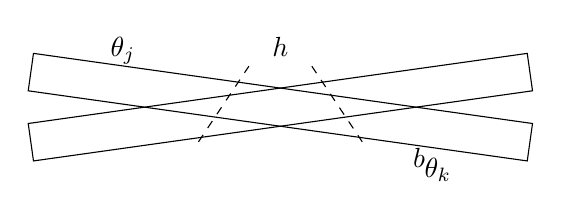
\begin{tikzpicture}[scale=0.8]
  % 两个交叉的长矩形
  \draw[rotate=8] (-4,-0.3) rectangle (4,0.3);
  \draw[rotate=-8] (-4,-0.3) rectangle (4,0.3);
  % 平行四边形 (交叠区域) 与虚线
  \draw[dashed] (-1.3,-0.55) -- (-0.5,0.65);
  \draw[dashed] (0.5,0.65) -- (1.3,-0.55);
  \node at (0,0.95) {$h$};
  \node at (2.2,-0.8) {$b$};
  \node at (-2.5,0.9) {$\theta_j$};
  \node at (2.5,-1.0) {$\theta_k$};
\end{tikzpicture}
\caption{相交矩形的几何与方向夹角}
\label{fig:8}
\end{figure}

\section{Kakeya 集}
\label{sec:7.2}

\begin{theorem}\label{thm:7.4}
\index{Kakeya 集 (Kakeya set)|emph}
\index{发芽 (sprouting)}
对每个 $k>k_0$, 存在集合 $E\subset\mathbb{R}^2$ 与互不相交的矩形族 $\{R_j\}$, 使得若 $\tilde{R}_j$ 是与 $R_j$ 全等、但沿 $R_j$ 最长边的方向平移所得的矩形对, 则
\[
\bigl|\tilde{R}_{j}\cap E\bigr|\geq\frac{1}{4}|R_{j}|,
\qquad
\frac{\sum|R_{j}|}{|E|}\geq C\log k.
\]
\end{theorem}

\begin{proof}
我们通过迭代一个称为``发芽'' (sprouting) 的过程得到集合 $E$. 这里的愿望是构造朝各个方向延伸、而公共交集很小的三角形. 我们先看看如何对两个三角形做到这一点. 设 $ABC$ 是图~\ref{fig:9} 中的三角形. 如图所示, 我们构造新三角形 $AA'M$ 与 $BB'M$: 把 $AC$ 延长到 $AA'$, 把 $BC$ 延长到 $BB'$. 设 $M$ 表示 $AB$ 的中点, 并作出三角形 $AA'M$ 与 $BB'M$.

这一过程构造了两个朝不同方向延伸的新三角形; 我们先证明没有增加多少新的面积. 设 $b$ 为 $AB$ 的底长, $h_{0}$ 为 $ABC$ 的高, $h_{1}$ 为 $AA'M$ 与 $BB'M$ 的高. 我们断言: 两个新三角形的并的面积至多为
\[
\frac{bh_{0}}{2}+2\,\frac{bh_{1}^{2}}{h_{0}}.
\]
设 $E$ 为直线 $AA'$ 与 $MB'$ 的交点, $F$ 为 $MA'$ 与 $BB'$ 的交点. 我们用三角形 $FEB'$ 与 $FEA'$ 的面积来估计三角形 $EB'C$ 与 $FA'C$ 的面积. 我们关注 $FEA'$. 由于 $FEA'$ 与 $MAA'$ 相似, 而 $FEC$ 与 $BAC$ 相似, 我们算得 $FEA'$ 的高为 $h_1+\frac{h_0h_1}{h_0+2h_1}<2h_1$, 并算得底
\[
|EF|=\frac{bh_{1}}{h_{0}+2h_{1}}<c\,\frac{bh_{1}}{h_{0}}.
\]
总面积被 $\frac{bh_{1}^{2}}{h_{0}}$ 控制. 同样的估计适用于 $FEB'$.

为构造集合 $E$, 我们从一个底为 $b$、高为 $h_{0}$ 的等腰三角形出发, 以高度增量 $\frac{h_0}{2}$ 使它发芽. 这得到两个三角形, 其中每一个再以高度增量 $\frac{h_0}{3}$ 发芽. 如此继续到第 $k$ 步. 我们有 $2^k$ 个三角形, 每个的底为 $b2^{-k}$, 高为 $h_0\sum_{i}\frac{1}{i}\approx h_0\log k$. 设 $E$ 是所有这些三角形的并. $E$ 的面积是多少? 在第 $i$ 步, 我们有 $2^i$ 个三角形; 取定其中一个. 它的高至少为 $h_0\log i$, 底至少为 $b2^{-i}$, 而高度增量为 $\frac{h_0}{i}$. 发芽过程增加的面积增量约为
\[
2\cdot\frac{b2^{-i}}{2}\cdot\frac{(h_0/i)^{2}}{h_0\log i}
=2\,\frac{b\,h_{0}\,2^{-i}}{i^{2}\log i}.
\]
由于有 $2^i$ 个三角形, 总增量为 $2\frac{bh_{0}}{i^{2}\log i}$, 于是 $E$ 的面积被
\[
\frac{bh_{0}}{2}+2\sum_{i}\frac{bh_{0}}{i^{2}\log i}<3bh_{0}
\]
控制.

现在我们对上面得到的 $2^k$ 个三角形构造相应的矩形 $R_j$. 图~\ref{fig:10} 画出了这一想法. 设 $ABC$ 是其中一个发芽后的三角形. 把直线 $AC$ 与 $BC$ 延长为直线 $GAC$ 与 $EBC$. 过点 $A$ 作 $DAC$ 的垂线, 直到它与 $EBC$ 交于 $F$. 线段 $AF$ 是 $R_j$ 的一条边. 另一条边是 $AG$, 其中 $G$ 的选取使得 $AC$ 的长度等于发芽三角形 $ABC$ 的高.

\begin{figure}[htbp]
\centering
\begin{minipage}[b]{0.45\textwidth}
\centering
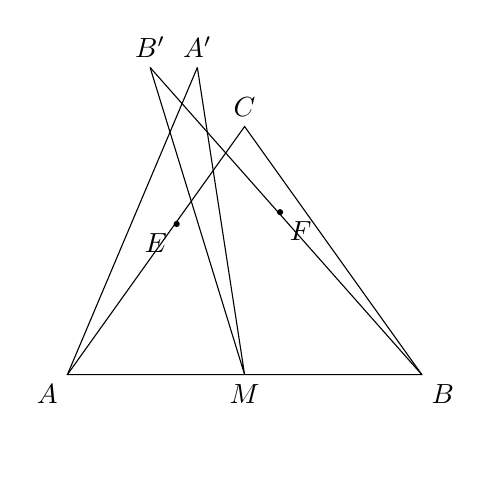
\begin{tikzpicture}[scale=0.75]
  % 图 9: 发芽
  \draw (0,0) node[below left] {$A$} -- (6,0) node[below right] {$B$} -- (3,4.2) node[above] {$C$} -- cycle;
  \draw (0,0) -- (2.2,5.2) node[above] {$A'$};
  \draw (6,0) -- (1.4,5.2) node[above] {$B'$};
  \draw (2.2,5.2) -- (3,0) node[below] {$M$} -- (1.4,5.2);
  \fill (1.85,2.55) circle (1.5pt) node[below left] {$E$};
  \fill (3.6,2.75) circle (1.5pt) node[below right] {$F$};
  \node at (3,-1.4) {};
\end{tikzpicture}
\caption{Besicovitch 三角形的发芽过程}
\label{fig:9}
\end{minipage}\hfill
\begin{minipage}[b]{0.45\textwidth}
\centering
\begin{tikzpicture}[scale=0.75]
  % 图 10: 矩形构造
  \draw (0.4,1.2) node[left] {$A$} -- (1.6,1.2) node[right] {$B$};
  \draw (0.4,1.2) -- (3.4,6.2) node[above] {$C$};
  \draw (1.6,1.2) -- (3.4,6.2);
  \draw (0.4,1.2) -- (-1.6,-3.4) node[left] {$G$};
  \draw (3.4,6.2) -- (-0.9,-3.2) node[below] {$E$};
  \draw (-1.6,-3.4) -- (0.9,0.9);
  \draw (0.75,0.95) arc (0:-60:0.45);
  \node at (1.35,0.55) {$\theta$};
  \fill (1.15,0.62) circle (1.5pt) node[below right] {$F$};
\end{tikzpicture}
\caption{沿发芽三角形构造细长矩形}
\label{fig:10}
\end{minipage}
\end{figure}

显然, 如此构造的诸 $R_j$ 互不相交, 长度为 $h_0\log k$, 宽度至多为 $b2^{-k}$. 我们还需要宽度的下界估计. 图~\ref{fig:10} 表明, 宽度由发芽三角形的细长程度控制. 若 $\theta$ 是 $AF$ 与 $AB$ 之间的夹角, 则 $\frac{AF}{AB}=\cos\theta$. 现在 $\theta=90-\angle(AB,AC)$, 而 $\angle(AB,AC)\geq 60$, 因为发芽过程增大了角部的角度, 而我们最初是一个等腰三角形. 于是 $\theta<30$ 且 $\cos\theta<\frac{\sqrt{3}AC}{2}=\frac{\sqrt{3}b2^{-k}}{2}$. 则
\[
\sum|R_{j}|=2^{k}|R_{0}|\geq 2^{k}\left(\frac{\sqrt{3}\,b\,2^{-k}}{2}\right)(h_{0}\log k),
\]
且
\[
\frac{\sum|R_{j}|}{|E|}\geq\frac{\sqrt{3}}{2}\cdot\frac{h_{0}b\log k}{3h_{0}b}\geq C\log k,
\]
正如所断言的.

最后, 我们估计
\[
|\tilde{R}_{j}\cap E|\geq\frac{1}{4}|\tilde{R}_{j}|.
\]
参考图~\ref{fig:11}. 显然
\begin{align*}
\bigl|\tilde{R}_{j}\cap E\bigr|&\geq\bigl|\tilde{R}_{j}\cap(ABC)\bigr|=\bigl|ABED\bigr| \\
&=\bigl|AFED\bigr|-\bigl|ABF\bigr|\geq\bigl|AFED\bigr|-\bigl|AFG\bigr|;
\end{align*}
在这个估计中我们用了 $AD=\text{height }ABC\leq AC$. 现在, 由于 $D$ 不等于 $E$, $|AFED|\geq\frac{1}{2}|\tilde{R}_j|$. 最后,
\begin{align*}
|AFG|&=\frac{1}{2}(AF)(FG)=(AF)^{2}\,\frac{\tan\theta}{2} \\
&\leq(AF)^{2}\,\frac{\tan\frac{\pi}{6}}{2}
\leq(AB)(AF)\,\frac{1}{2\sqrt{3}} \\
&=\frac{b2^{-k}}{2\sqrt{3}}(AF)\leq h_{0}\,\frac{\log k}{4}\,(AF)=\frac{1}{4}|\tilde{R}_{j}|.
\end{align*}
于是,
\[
|\tilde{R}_{j}\cap E|\geq\frac{1}{2}|\tilde{R}_{j}|-\frac{1}{4}|\tilde{R}_{j}|.
\]
\end{proof}

\begin{figure}[htbp]
\centering
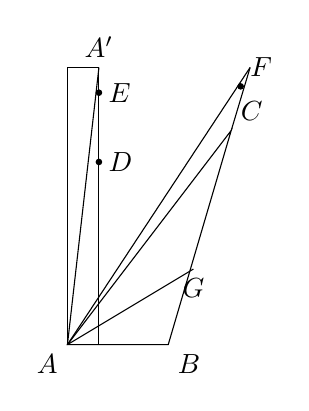
\begin{tikzpicture}[scale=0.8]
  % 图 11: R̃_j 与三角形 ABC
  \draw (0,0) node[below left] {$A$} -- (1.6,0) node[below right] {$B$}
        -- (2.6,3.4) node[above right] {$C$} -- cycle;
  \draw (0,0) -- (0.5,4.4) node[above] {$A'$};
  \draw (0,0) rectangle (0.5,4.4);
  \fill (0.5,2.9) circle (1.5pt) node[right] {$D$};
  \fill (0.5,4.0) circle (1.5pt) node[right] {$E$};
  \draw (0,0) -- (2.9,4.4);
  \draw (2.6,3.4) -- (2.9,4.4);
  \fill (2.75,4.1) circle (1.5pt) node[above right] {$F$};
  \draw (0,0) -- (2.0,1.2) node[below] {$G$};
\end{tikzpicture}
\caption{矩形与 Kakeya 集合交集的面积下界}
\label{fig:11}
\end{figure}

\begin{theorem}\label{thm:7.5}
\index{乘子!球的乘子问题 (multiplier problem for the ball)}
$T_0$ 在 $L^p(\mathbb{R}^n)$ 上无界, 若 $n>1$ 且 $p\neq 2$.
\end{theorem}

\begin{proof}
设 $T_0$ 有界; 我们可以假设 $p>2$; 我们将证明: 对每个 $k>k_0$,
\[
{}_{p}\|T_{0}\|>C(\log k)^{\frac{1}{2}-\frac{1}{p}}.
\]
取定 $k$, 我们如定理~\ref{thm:7.4} 那样构造 Kakeya 集 $E$ 与矩形 $R_j$. 若 $v_j$ 是 $R_j$ 最长边的方向, 我们令 $f_j=\chi_{R_j}$, 并用定理~\ref{thm:7.2} 得到
\[
\Bigl\|\Bigl(\sum|H_{j}f_{j}|^{2}\Bigr)^{\frac{1}{2}}\Bigr\|_{p}
\leq{}_{p}\|T_{0}\|\,\Bigl\|\Bigl(\sum|f_{j}|^{2}\Bigr)^{\frac{1}{2}}\Bigr\|_{p}.
\]
我们将证明: 对 $x\in\tilde{R}_j$, 有 $|H_jf_j(x)|\geq C$. 由此可得
\begin{align*}
C\sum|R_{j}|&=C\sum|\tilde{R}_{j}|\leq C\sum|\tilde{R}_{j}\cap E|
=C\sum\int_{\tilde{R}_{j}\cap E}\leq\sum\int_{\tilde{R}_{j}\cap E}|H_{j}f_{j}|^{2} \\
&\leq\sum\int_{E}|H_{j}f_{j}|^{2}=\int_{E}\sum|H_{j}f_{j}|^{2}
\leq|E|^{1-\frac{2}{p}}\left(\int_{E}\Bigl(\sum|H_{j}f_{j}|^{2}\Bigr)^{\frac{p}{2}}\right)^{\frac{2}{p}} \\
&\leq|E|^{1-\frac{2}{p}}\,{}_p\|T_{0}\|\Bigl\|\Bigl(\sum|H_{j}f_{j}|^{2}\Bigr)^{\frac{1}{2}}\Bigr\|_{p}^{2} \\
&\leq|E|^{1-\frac{2}{p}}\,{}_p\|T_{0}\|\Bigl\|\Bigl(\sum|f_{j}|^{2}\Bigr)^{\frac{1}{2}}\Bigr\|_{p}^{2} \\
&\leq|E|^{1-\frac{2}{p}}\,{}_p\|T_{0}\|\Bigl(\sum|R_{j}|\Bigr)^{\frac{2}{p}}.
\end{align*}
分离出 ${}_p\|T_0\|$, 得
\[
{}_{p}\|T_{0}\|\geq C\left(\frac{\sum|R_{j}|}{|E|}\right)^{1-\frac{2}{p}}
\geq C(\log k)^{1-\frac{2}{p}}.
\]
为完成证明, 我们需要估计 $H_jf_j$. 我们注意到这些估计在旋转与平移下不变, 于是可以假设 $v_j=(0,1)$, $R_j=(0,a)\times(0,b)$. 则
\[
\chi_{P_{j}}(\xi_{1},\xi_{2})=\frac{1-i\,(i\,\mathrm{sign}\,\xi_{2})}{2},
\]
于是
\[
H_{j}=\frac{I\times I-i\,I\times H}{2}.
\]
由于 $f_{j}=\chi_{R_{j}}$ 是实的,
\[
|H_{j}f_{j}|\geq\frac{1}{2}\bigl|(I\times H)f_{j}\bigr|.
\]
但
\begin{align*}
(I\times H)f_{j}(x_{1},x_{2})
&=\iint\delta(x_{1}-y_{1})\,\chi_{(0,a)}(y_{1})\,\frac{\chi_{(0,b)}(y_{2})}{x_{2}-y_{2}}\,dy_{1}\,dy_{2} \\
&=\chi_{(0,a)}(x_{1})\int\frac{\chi_{(0,b)}(y_{2})}{x_{2}-y_{2}}\,dy_{2}.
\end{align*}
现在 $\tilde{R}_j=(0,a)\times(-b,0)\cup(0,a)\times(b,2b)$, 于是 $(x_1,x_2)\in\tilde{R}_j$ 蕴含 $\chi_{(0,a)}=1$ 且 $|x_2-y_2|<2b$, 从而
\[
|H_{j}f_{j}(x_{1},x_{2})|\geq\left|\int\frac{\chi_{(0,b)}(y_{2})}{2b}\,dy_{2}\right|=\frac{1}{2}. \qedhere
\]
\end{proof}

\begin{corollary}\label{cor:7.6}
$T_0$ 在 $L^p(\mathbb{R}^n)$ 上无界, 若 $n>1$ 且 $p\neq 2$.
\end{corollary}

\begin{proof}
若 $T_0$ 在 $L^p$ 上有界, 我们可以把 $\mu_0=\chi_B$, $B=\{\xi \mid |\xi|<1\}$ 限制到 $\mathbb{R}^n$ 中的平面上. 由定理~\ref{thm:1.23}f), 这些限制几乎处处都是 $L^p(\mathbb{R}^2)$ 的乘子. 现在取垂直于 $\xi_1$ 轴的平面, $\mu_0$ 在这些平面上的限制是一列圆盘. 其中至少有一个必是 $L^p(\mathbb{R}^2)$ 的乘子, 这与定理~\ref{thm:7.5} 矛盾.
\end{proof}

\essayhead{ess:7.7}{另一种证明}

在这一短论中, 我们勾画~\ref*{cor:7.6} 的一个更符合``反例应当长什么样''的直观的证明.

我们预计 $\hat{f}_j$ 是以单位向量 $v_j$ 为中心、大小为 $\delta\times\delta^2$ 的矩形的特征函数; 反例函数 $f_j$ 应当是大小为 $N\times N^2$ 的矩形乘以指数 $e^{2\pi iv_jx}$.

\begin{lemma}\label{lem:7.8}
对每个 $\gamma>0$ 与 $k>k_0$, 存在 $N_k$、集合 $E$ 与 $2^k$ 个互不相交的矩形 $\{R_j\}$, 满足:
\begin{enumerate}[label=\arabic*)]
\item 每个 $R_j$ 的较长边的长度为 $N_k^2$; 较短边被一个常数倍上下界住, 即与 $N_k$ 可比.
\item $|E|\leq C(\log\log N_k)^{-1}\sum|R_j|$.
\item 若 $\bar{R}_j$ 是 $R_j$ 沿其最长方向平移距离 $(1+\gamma)N_k^2$ 所得的矩形, 则 $|\bar{R}_j\cap E|\geq C|R_j|$.
\item $\lim_{k\to\infty}N_k=\infty$.
\end{enumerate}
\end{lemma}

\begin{proof}
证明与定理~\ref{thm:7.4} 几乎相同. 起始三角形被赋予初始高度 $2^{2k}\log k$, 并以第 $i$ 步高度增量 $\frac{2^{2k}\log k}{i}$ 发芽. 经过 $k$ 步, 三角形的高为 $N_k^2=2^{2k}\log^{2}k$. 旧的 $R_j$ 照旧构造, 而新的 $R_j$ 由把旧的 $R_j$ 沿远离 $E$ 的方向平移 $\gamma N_k$ 个单位得到, 这些就是我们所说的 $R_j$. 于是 $\bar{R}_j$ 就是原来的 $\tilde{R}_j$, 从而享有同样的估计.
\end{proof}

\par\vspace{1.2em}
{\noindent{\songfont\bfseries 短论~\ref*{ess:7.7} (续)}\par}
\vspace{0.4em}

为了让计算 manageable, 我们将使用一个更简单的模型; 我们不用正确的
\[
K_{0}(x)=\frac{\cos\bigl(2\pi|x|-\frac{3\pi}{4}\bigr)}{|x|^{\frac{3}{2}}}+O\Bigl(|x|^{-\frac{5}{2}}\Bigr),
\]
而用
\[
K(x)=\frac{e^{i|x|}}{|x|^{\frac{3}{2}}}.
\]
从关于 $K$ 的否定信息过渡到关于 $K_{0}$ 的信息是不可能的, 但对 $K_{0}$ 的完整处理要把 $\cos$ 的加法公式用上许多次, 以至于那些不重要的误差项会像苍蝇一样累积. 我们就做 $K$.

如同定理~\ref{thm:7.4} 的证明, 只需证明 $|K\star f_j(x)|\geq c$ 对 $x\in\bar{R}_j$ 成立. 利用~\ref*{sec:6.1} 开头的分析, 我们可以直观地完成计算. 由于 $f_j=e^{iv_j\cdot y}\chi_{R_j}(y)$ 且 $x\in\bar{R}_j$, $x$ 远离 $f_j$ 的支集, 于是
\[
K\star f_{j}(x)\approx\frac{e^{i|x|}}{|x|^{\frac{3}{2}}}\,\hat{f}_{j}\Bigl(\frac{x}{|x|}\Bigr).
\]
现在 $\hat{f}_j$ 是以 $v_j$ 为中心的矩形的特征函数乘以齐性因子 $N^{3}$, 至少对所有使 $\frac{x}{|x|}$ 落在 $\hat{f}_j$ 的支集内的 $x$ 如此. 这发生在 $\bigl|\frac{x}{|x|}-v_j\bigr|<\frac{1}{N}$ 时, 而当 $x\in\bar{R}_j$ 时这是成立的. 于是
\[
|K\star f_{j}|\approx\frac{N^{3}}{|x|^{\frac{3}{2}}},
\]
但 $|x|\approx R_j\ \text{的最长边}=\gamma N^2$, 故
\[
|K\star f_{j}|\approx\frac{C}{\gamma^{\frac{3}{2}}}.
\]
让这个计算严格化是相当容易的; 我们从~\ref*{prop:6.1} 中估计的一个严格版本开始. 设 $w_j$ 是垂直于 $v_j$ 的单位向量; 若 $x\in\bar{R}_j$, $y\in R_j$, $\gamma>2$, 则
\begin{gather*}
\gamma N^{2}<|x-y|<3\gamma N^{2}, \\
\gamma N^{2}\leq\bigl|(x-y)\cdot v_{j}\bigr|<2\gamma N^{2}, \\
\bigl|\bigl(x-y\bigr)\cdot w_{j}\bigr|<\sqrt{2}\,N.
\end{gather*}
则
\begin{align*}
|x-y|&=\left(\bigl[(x-y)\cdot v_{j}\bigr]^{2}+\bigl[(x-y)\cdot w_{j}\bigr]^{2}\right)^{\frac{1}{2}} \\
&=\bigl|(x-y)\cdot v_{j}\bigr|\left(1+\frac{\bigl[(x-y)\cdot w_{j}\bigr]^{2}}{\bigl[(x-y)\cdot v_{j}\bigr]^{2}}\right)^{\frac{1}{2}}.
\end{align*}
现在对 $\sqrt{1+x}$ 在 $0$ 附近、以及对 $e^{ix}$ 在 $0$ 附近使用 Taylor 展开, 我们得到
\[
e^{i|x-y|}=e^{i(x-y)\cdot v_{j}}+Error,
\]
其中
\begin{align*}
|Error|&\leq C\max\frac{\bigl[(x-y)\cdot w_{j}\bigr]^{2}}{\bigl|(x-y)\cdot v_{j}\bigr|}
\leq\frac{C_2N^{2}}{\gamma N^{2}}=\frac{C}{\gamma}.
\end{align*}
现在我们选取 $E$ 的定向使 $(x-y)\cdot v_j\geq 0$; 则
\[
|K\star f_{j}(x)|
\geq\left|\int\frac{e^{i(x-y)\cdot v_{j}}}{|x-y|^{\frac{3}{2}}}\,e^{iv_{j}\cdot y}\chi_{R_{j}}(y)\,dy\right|
-\int_{R_{j}}\frac{Error}{|x-y|^{\frac{3}{2}}}\,dy.
\]
第一项是
\[
\int_{R_{j}}|x-y|^{-\frac{3}{2}}\,dy\geq\bigl(3\gamma N^{2}\bigr)^{-\frac{3}{2}}|R_{j}|=C\gamma^{-\frac{3}{2}}.
\]
第二项被下式从上方控制:
\[
\frac{C}{\gamma}\int_{R_{j}}|x-y|^{-\frac{3}{2}}\,dy
=\frac{C}{\gamma}\cdot\frac{C}{(2\gamma)^{\frac{3}{2}}}\cdot\frac{|R_{j}|}{N^{3}}
\leq\frac{C}{\gamma^{\frac{5}{2}}}.
\]
若 $\gamma$ 充分大, 第二项是第一项的一半, 于是
\[
|K\star f_{j}|\geq\frac{C}{\gamma^{\frac{3}{2}}}.
\]

\section{评注与推广}
\label{sec:7.3}

\noindent (7.1):\quad 定理~\ref{thm:7.1} 取自 Zygmund~\cite{zygmund}; 这里的证明对混合 $f$ 的实部与虚部的算子 $T$ 不适用. Paley 展示了如何用复的 Gaussian 函数对不令人愉快的 $T$ 建立结果. 由于我们实际上处理的是 $(f_1,f_2,\ldots,f_k)$ 上的 Euclid 范数, 这一整个课题被称为``向量值不等式''.

\noindent (7.2):\quad 定理~\ref{thm:7.2} 归功于 Yves~Meyer, 该结果通常称为``Meyer 引理''. 它可以应用于圆盘之外的集合; 事实上, 若 $C$ 是 $\mathbb{R}^2$ 中法方向只有 $N$ 个的凸集, 那么关于这些方向上 Hilbert 变换的 Meyer 引理便可适用. 这将给出 $N$ 边形特征函数的 $L^p$ 乘子范数的下界. 类似地, Meyer 引理可用于证明: 乘子 $|1-|\xi|^2|^{it}$ 的 $L^p$ 有界性导致对卷积核 $K_j(x)=|x\cdot v_j|^{-1-it}$ 的向量值不等式.

Meyer 引理最深远的应用是在 A.~C\'ordoba 与 R.~Fefferman 的理论中, 它把极大函数与乘子联系起来.

\noindent (7.4):\quad Kakeya 集最初是为解决平面上的一个几何问题而构造的. 考虑长度为 $1$ 的线段 $I$; 设 $E$ 是一个集合. 只要不离开 $E$, 我们可以随意旋转与平移 $I$. 使 $I$ 能完整旋转 $360^\circ$ 的 $E$ 的最小面积是多少? 利用 Kakeya 集可以证明: 对每个 $\epsilon$, $|E|$ 都可以做得小于 $\epsilon$. 精彩的阐述见 de Guzm\'an~\cite{deguzman}. 相关推广在 Cunningham~\cite{cunningham} 中讨论.

Kakeya 集的种种变体可用于分析 $\mathbb{R}^2$ 中其他几何--分析问题, 特别是积分的微分. 问题是: 对 $\mathbb{R}^2$ 上的函数, 基于对方形或球作平均构造一个极大函数; 一维的想法给出弱 $L^1$ 与 $L^p$ 界. 但若试图沿任意方向对矩形作平均, Kakeya 集技术表明上确界是无穷. 参见 de Guzm\'an~\cite{deguzman}.

\noindent (7.4):\quad 这个结果归功于 C.~Fefferman. 显然, 同样的想法可以推广到任何沿一个连续的方向集合具有间断的乘子; 特别地, 推广到径向函数的跳跃间断. 振荡型间断的情形仍未解决.

\noindent (7.7):\quad 这里的替代证明源自 C.~Fefferman~\cite{fefferman-ball} 中的概要; 另见~\cite{kenig-tomas}. 计算技巧的意义在于, 即使 Meyer 引理不适用时它们仍然适用; 见 Ruiz~\cite{cordoba-flp}.
